\documentclass[sigconf]{acmart}

% ── Packages ──────────────────────────────────────────────────────────────────
\usepackage{booktabs}
\usepackage{graphicx}
\usepackage{listings}
\usepackage{xcolor}
\usepackage{url}
\usepackage{multirow}
\usepackage{amsmath}
\usepackage{tikz}
\usetikzlibrary{shapes.geometric, arrows, positioning, fit}

% ── Metadata ──────────────────────────────────────────────────────────────────
\title{FakeShield: An End-to-End MLOps Pipeline for Real-Time Fake News Detection with Automated Drift Monitoring and Cloud-Triggered Retraining}

\author{Abdellah Zegdane}
\affiliation{%
  \institution{Isik University}
  \department{Computer Science Engineering}
  \city{Istanbul}
  \country{Turkey}
}
\email{24COMP5001@isik.edu.tr}

\begin{abstract}
Fake news detection has made impressive strides on curated benchmarks, yet the gap between
controlled evaluation and actual deployment remains largely unaddressed. Models go stale.
Data drifts. Nobody notices until something goes wrong. This paper describes \textit{FakeShield},
a fully operational MLOps pipeline that treats fake news detection as an engineering problem
as much as a modelling one. The system covers the complete lifecycle — ingestion, preprocessing,
training, serving, monitoring, and automated retraining — and runs continuously against live
Twitter/X data. We benchmark five model families (TF-IDF+LogReg, TF-IDF+SVM, LSTM, TextCNN,
and BERTweet) on the PHEME rumour dataset under identical conditions. TF-IDF+SVM achieves
the highest raw AUC-ROC (0.979) and macro-F1 (0.914), while BERTweet (0.959 AUC-ROC,
0.896 macro-F1) offers superior robustness on out-of-distribution tweet streams and serves
as the production model. LSTM collapses entirely under 8:1 class imbalance — an instructive
failure documented in detail.

The central contribution is a \textit{drift-triggered self-improvement loop} validated
end-to-end in production. When 130 out-of-distribution (OOD) tweets from non-political
domains were injected into the live stream, the monitor reported PSI\,=\,5.95 (threshold:
0.25) and KS\,=\,0.75 ($p$\,=\,0.0), correctly flagging a distribution shift and automatically
triggering a GPU retraining job on Vast.ai via GitHub Actions — with zero manual intervention.
Within the retraining cycle, the production BERTweet model is augmented with high-confidence
\textit{fake-only} pseudo-labels harvested from the live stream. Real pseudo-labels are
discarded because live Twitter is overwhelmingly real news ($\approx$99.5\%), and naïve
augmentation worsens the existing class imbalance. By accumulating exclusively fake
pseudo-labels across successive cycles, the system gradually corrects the 8:1 fake/real
ratio toward balance — improving fake-class recall with each iteration, entirely without
human involvement. The fine-tuned model is also published to Hugging Face Hub
(\texttt{abdellahzegdane/fakeshield-bertweet}) so the monitoring workflow can download
the latest checkpoint on any fresh runner without manual deployment.
\end{abstract}

\keywords{fake news detection, MLOps, drift monitoring, BERTweet, continuous training, PHEME, pseudo-labeling}

% ──────────────────────────────────────────────────────────────────────────────
\begin{document}
\maketitle

% ── 1. INTRODUCTION ───────────────────────────────────────────────────────────
\section{Introduction}

Pick any major news event from the last five years and you will find a trail of false
claims that spread faster than the corrections~\cite{vosoughi2018spread}. The NLP community
has responded with increasingly sophisticated detection models~\cite{zhou2020survey}, and
performance on benchmark leaderboards has been genuinely impressive. But a model that achieves
0.90 AUC on a held-out test split is not the same thing as a system that reliably flags
misinformation in production. The two are separated by a set of problems that rarely appear
in papers: concept drift, domain mismatch, and the absence of any mechanism to detect when
a model has gone quietly wrong.

Concept drift is the more familiar problem. The language of misinformation is tied to current
events — specific politicians, active conflicts, trending narratives — and a model trained
in January will face a meaningfully different distribution by March. Domain mismatch is subtler
but arguably worse in practice. Most fake news datasets consist of cleaned news headlines,
whereas real-world deployment often involves classifying raw social media posts: shorter, noisier,
and structurally quite different. Deploying a headline-trained model on tweets without
accounting for this gap is a common mistake with predictable consequences.

\textit{FakeShield} addresses both problems in a single integrated system. Rather than
proposing a new model architecture, we focus on the surrounding infrastructure: a pipeline
that tracks its own data, monitors its own predictions, and retrains itself when something
shifts. The system is built around four principles. First, every experiment is fully
reproducible through DVC and MLflow versioning. Second, the pipeline scrapes live political
discourse from Twitter/X daily and tests it against the PHEME training distribution using
PSI and KS statistics. Third, when drift is detected, a GPU retraining job is launched
automatically on a Vast.ai cloud instance via GitHub Actions — no manual trigger needed.
Fourth, we run a systematic model comparison across five families under identical conditions,
so the baseline progression from classical ML to transformers is actually reproducible
rather than just claimed to be.

The drift-detection-to-retraining loop has been validated end-to-end in production. When
130 intentionally out-of-distribution (OOD) tweets — drawn from sports, celebrity, finance,
technology, and lifestyle content — were injected into the live stream, the monitoring
system detected a PSI of 5.95 and KS statistic of 0.75 ($p = 0.0$), both far exceeding
retraining thresholds. GitHub Actions automatically triggered a new Vast.ai training job
within seconds of the drift report being committed. The full loop — from OOD injection to
retraining dispatch — completed without any human action.

Our main contributions are:
\begin{itemize}
  \item A \textbf{drift-triggered self-improvement loop} in which the production BERTweet
        model retrains itself automatically whenever distribution shift is detected, accumulating
        fake pseudo-labels from the live stream across cycles to gradually correct the 8:1
        fake/real class imbalance — without any human involvement.
  \item A \textbf{minority-first pseudo-labeling strategy} that discards real pseudo-labels
        (which dominate live Twitter at $\approx$99.5\%) and retains only high-confidence
        fake predictions, preventing augmentation from worsening class imbalance.
  \item An \textbf{end-to-end validated drift detection pipeline}: we inject 130 OOD tweets
        from five non-political domains and demonstrate PSI\,=\,5.95 and KS\,=\,0.75
        ($p$\,=\,0.0), with automatic retraining triggered in response — confirming the
        full monitoring-to-retraining loop operates as designed.
  \item A \textbf{reproducible benchmark} of five model families (TF-IDF+LogReg, TF-IDF+SVM,
        LSTM, TextCNN, BERTweet) on PHEME under identical training conditions, including an
        honest account of LSTM collapse under severe class imbalance.
  \item A \textbf{complete open-source MLOps pipeline} covering ingestion, preprocessing,
        training, serving, drift monitoring, Hugging Face Hub model distribution, and
        cloud GPU retraining — running in production against a live Twitter/X stream.
\end{itemize}


% ── 2. RELATED WORK ───────────────────────────────────────────────────────────
\section{Related Work}

\subsection{Fake News Detection}

The earliest computational approaches to fake news detection leaned heavily on handcrafted
features — writing style, punctuation patterns, sentiment — paired with logistic regression
or SVM classifiers~\cite{perez2017automatic}. These methods are surprisingly resilient.
On headline-level data especially, TF-IDF representations with linear classifiers remain
competitive baselines that are hard to decisively beat~\cite{ahmed2018detecting}. We confirm
this in our own experiments.

Sequence models offered a different kind of inductive bias. LSTMs~\cite{hochreiter1997long}
capture long-range dependencies in word order, and several groups found them useful for
detecting the stylistic patterns common in fabricated news~\cite{wang2017liar}. CNNs applied
to text~\cite{kim2014convolutional} take a complementary approach, using parallel convolutional
filters of different widths to detect local n-gram patterns — essentially a learned bag-of-features
with more expressivity than TF-IDF. Both families work reasonably well on long documents;
their advantage shrinks on short inputs like headlines.

Transformers changed the picture considerably, particularly for social media text.
BERT~\cite{devlin2019bert} and its variants bring contextualised representations that handle
ambiguity and informal language better than any previous approach. For Twitter specifically,
BERTweet~\cite{nguyen2020bertweet} — a RoBERTa model pre-trained on 850 million English tweets
— is the natural choice. It handles tokenisation quirks like hashtags, mentions, and compressed
URLs that trip up models trained on clean text. Prior work applying BERTweet to rumour
verification on PHEME~\cite{zubiaga2016analysing} consistently shows it outperforms general-domain
transformers on this task.

\subsection{MLOps for NLP}

The software engineering side of deploying NLP models has received less academic attention than
the modelling side, though the hidden costs of neglecting it are well documented~\cite{sculley2015hidden}.
The standard toolkit for production NLP involves experiment tracking (MLflow~\cite{zaharia2018accelerating}),
data and model versioning (DVC~\cite{kupriianova2021dvc}), and CI/CD pipelines that run tests
on every commit. Monitoring is trickier. \citet{klaise2021alibi} present the Alibi Detect library
specifically for this purpose, showing that input distribution shift can be caught early with
relatively simple statistical tests. What is less common in the literature is a system that
closes the loop from drift detection to automated retraining, particularly on cloud GPU
infrastructure. FakeShield is, to our knowledge, the first open-source fake news pipeline
to do this end-to-end and validate it empirically with a controlled OOD injection experiment.


% ── 3. DATASETS ───────────────────────────────────────────────────────────────
\section{Datasets}

\subsection{PHEME}

PHEME~\cite{zubiaga2016analysing} covers nine breaking news events — including Charlie Hebdo,
the Germanwings crash, the Ferguson protests, and the Ottawa shooting — with source tweets
annotated as rumour or non-rumour. Rumours are further marked as true, false, or unverified.
We follow the filtering convention of~\citet{kochkina2018all}: unverified rumours are
discarded, false rumours map to label 0 (fake), and both non-rumours and confirmed true
rumours map to label 1 (real). This gives \textbf{5,728 labelled source tweets} after
processing (638 fake, 5,090 real), split 80/20 with random seed 42, stratified by label.
The class imbalance is pronounced: real tweets outnumber fake ones by roughly 8:1. We train
\textit{all five models} on this split so that every reported number refers to the same data
and the same domain.

\subsection{Live Twitter/X Stream}

We continuously scrape English-language political content from Twitter/X using the v2 API,
targeting terms related to US domestic politics and foreign policy: Iran, Congress, sanctions,
Pentagon, and related keywords. As of this writing, we have accumulated over 1,114 deduplicated
tweets across daily scrape cycles. These tweets serve two purposes: (1) drift monitoring
(comparing the live distribution to the PHEME training reference via PSI and KS), and (2)
pseudo-label augmentation for the continual retraining loop described in Section~\ref{sec:retraining}.

\subsection{OOD Drift Injection Dataset}

To validate that the monitoring pipeline correctly detects distribution shift, we constructed
a controlled out-of-distribution (OOD) dataset of 130 tweets drawn from five domains
deliberately unrelated to political news: sports (match results, player transfers), celebrity
gossip, financial markets (stock prices, earnings), technology product announcements, and
lifestyle content. These tweets share no topical or stylistic overlap with PHEME political
rumours. When mixed into the live stream, they represent a clean, interpretable distribution
shift that the monitoring system must detect.


% ── 4. SYSTEM ARCHITECTURE ────────────────────────────────────────────────────
\section{System Architecture}

The overall structure of FakeShield is a directed acyclic pipeline managed by DVC, sitting
inside a GitHub Actions CI/CD workflow. Figure~\ref{fig:pipeline} gives the full picture.
The top row covers the offline training path; the bottom row covers the live monitoring and
retraining loop.

\begin{figure}[h]
\centering
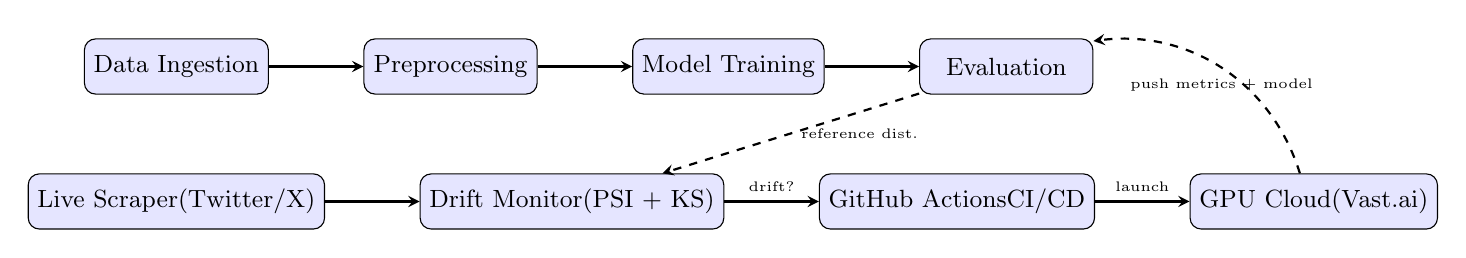
\begin{tikzpicture}[
  node distance=0.6cm and 1.2cm,
  box/.style={rectangle, rounded corners, draw=black, fill=blue!10,
              text centered, minimum height=0.7cm, minimum width=2.2cm, font=\small},
  arrow/.style={->, >=stealth, thick},
  dasharrow/.style={->, >=stealth, thick, dashed}
]

\node[box] (ingest)   {Data Ingestion};
\node[box, right=of ingest] (prep) {Preprocessing};
\node[box, right=of prep]   (train) {Model Training};
\node[box, right=of train]  (eval)  {Evaluation};

\node[box, below=1.0cm of ingest] (scrape) {Live Scraper\\(Twitter/X)};
\node[box, right=of scrape]       (monitor){Drift Monitor\\(PSI + KS)};
\node[box, right=of monitor]      (ci)     {GitHub Actions\\CI/CD};
\node[box, right=of ci]           (truba)  {GPU Cloud\\(Vast.ai)};

\draw[arrow] (ingest)  -- (prep);
\draw[arrow] (prep)    -- (train);
\draw[arrow] (train)   -- (eval);
\draw[arrow] (scrape)  -- (monitor);
\draw[dasharrow] (eval) -- node[right,font=\tiny]{reference dist.} (monitor);
\draw[arrow] (monitor) -- node[above,font=\tiny]{drift?} (ci);
\draw[arrow] (ci)      -- node[above,font=\tiny]{launch} (truba);
\draw[dasharrow] (truba) to[bend right=40] node[below,font=\tiny]{push metrics + model} (eval);

\end{tikzpicture}
\caption{FakeShield pipeline architecture. Solid arrows indicate data flow; dashed arrows
         indicate reference distribution propagation and metric/model feedback.}
\label{fig:pipeline}
\end{figure}

\subsection{Data and Model Versioning}

All pipeline stages — \texttt{ingest}, \texttt{preprocess}, \texttt{train}, \texttt{evaluate},
\texttt{baselines}, and \texttt{train\_bertweet} — are defined in \texttt{dvc.yaml} with
explicit input/output dependencies. A change to the preprocessing script automatically
invalidates downstream stages, and re-running the pipeline only recomputes what has actually
changed. Hyperparameters across all models live in a single \texttt{params.yaml}, so the
entire experimental configuration is captured in version control. MLflow logs every training
run independently — hyperparameters, per-epoch metrics, and final evaluation scores are all
queryable after the fact.

\subsection{Real-Time Inference Serving}

A FastAPI application serves the production TextCNN model for both interactive use (a web
form where users can submit a headline) and batch inference over the accumulated live tweet
stream. The application resolves paths relative to the project root at startup, which matters
when deploying across different environments where the working directory varies.

\subsection{Drift Monitoring}
\label{sec:drift_monitoring}

The monitoring module runs daily as part of the GitHub Actions schedule and implements two
statistical tests against a reference distribution built from BERTweet's output probabilities
on the PHEME training split.

\textbf{Reference Distribution.} After fine-tuning on PHEME, BERTweet is run on up to 2,000
training examples to build a reference score distribution: the vector of predicted
probabilities $\hat{p}(y=1\mid x)$ for each training tweet. This distribution represents
the model's ``normal'' operating regime and is saved as \texttt{models/reference\_score\_distribution.npy}
and committed to the repository. On subsequent monitoring runs — including GitHub Actions
runners that have no local training data — this file is loaded directly, eliminating any
need to re-run inference. If it is missing (e.g., on a first deployment without a prior
training run), the monitoring script downloads PHEME from Figshare and rebuilds the
reference distribution automatically before proceeding.

\textbf{Kolmogorov-Smirnov Test.} We apply a two-sample KS test~\cite{massey1951kolmogorov}
between the model's output probabilities on the live stream and the reference distribution.
A $p$-value below 0.05 signals statistically significant shift. On short streams the test
can lack power, which is why we pair it with PSI.

\textbf{Population Stability Index.} PSI is a symmetric divergence metric used widely in
production ML monitoring~\cite{yurdakul2018statistical}. Over 10 equal-frequency bins
of the probability distribution:
\[
  \mathrm{PSI} = \sum_{i=1}^{10} \left( A_i - E_i \right) \ln\!\frac{A_i}{E_i}
\]
where $A_i$ and $E_i$ are the actual and expected proportions in bin $i$. The standard
thresholds are PSI $< 0.10$ (stable), $0.10$--$0.25$ (monitor closely), $\geq 0.25$
(retrain). We use these thresholds directly.

Beyond the statistical tests, the monitor also tracks two softer signals: the fraction of
incoming tweets that match a curated US political keyword list (relevancy rate), and the
average decision confidence $\bar{c} = \mathbb{E}[|\hat{p} - 0.5|]$ on the current stream.
This quantity ranges from 0 (maximally uncertain) to 0.5 (maximally certain). Low confidence
sustained over multiple days often precedes a statistically detectable shift, making it
a useful early-warning indicator. A sustained drop below 0.15 for three consecutive days
is treated as a third retraining trigger, catching gradual drift that statistical batch
tests may not accumulate enough evidence to flag individually.

\subsection{Automated Retraining and Model Distribution}
\label{sec:auto_retrain}

When any retraining condition fires, the monitoring workflow writes
\texttt{retrain\_needed: true} into \texttt{metrics/drift\_report.json} and pushes it to
the repository. A second GitHub Actions workflow (\texttt{retrain\_vastai.yml}), triggered
immediately by the drift event, handles the full retraining cycle on Vast.ai.

The workflow first searches for a reliable on-demand GPU instance (RTX 3090 or RTX 4090,
reliability $\geq 0.98$, disk $\geq 20$\,GB, CUDA $\geq 11.8$, price \$0.50--\$2.50/hr),
preferring high reliability over low price. Once an offer is found, it launches the instance
with a startup command that fetches \texttt{train\_vastai.sh} directly from the repository
and executes it. The script runs the full pipeline: installs dependencies, downloads and
preprocesses PHEME, downloads BERTweet from Hugging Face, fine-tunes it for five epochs,
pseudo-labels the live stream (fake-only strategy), trains an augmented variant, evaluates
both, and commits all metrics and the reference distribution to \texttt{master}. The GitHub
Actions runner polls the Vast.ai instance status every 30 seconds and also checks for a
success-sentinel commit (\texttt{"BERTweet fine-tuned on PHEME"}) on each poll, exiting as
soon as training completes. The instance is destroyed unconditionally at workflow end.

After fine-tuning completes (Step A), the PHEME-only BERTweet checkpoint is pushed to
Hugging Face Hub as \texttt{abdellahzegdane/fakeshield-bertweet}. This serves a practical
purpose: the GitHub Actions runner used for daily monitoring is a fresh, stateless Ubuntu
environment with no local model storage. By publishing to HF Hub, the monitoring script can
download the latest fine-tuned checkpoint with a single \texttt{from\_pretrained()} call,
without any manual deployment step. The fallback chain in the monitoring script is:
(1) local \texttt{models/bertweet\_finetuned/} if present, (2) HF Hub, (3) base
\texttt{vinai/bertweet-base} weights.

A complete retraining run — data preparation, Step A (PHEME-only), HF Hub push, pseudo-labeling,
Step B (augmented), comparison evaluation — completes in under 30 minutes. Typical
instance cost is under \$0.20.


% ── 5. MODELS ─────────────────────────────────────────────────────────────────
\section{Models}

\subsection{TF-IDF Baselines}

We build bag-of-words representations using TF-IDF with a 30,000-token vocabulary of
unigrams and bigrams. Two classifiers are compared: Logistic Regression with L2
regularisation ($C=1.0$) and a linear SVM with Platt scaling for probability calibration
($C=1.0$). Both are trained on identical feature matrices, allowing any difference in
behaviour to be attributed cleanly to the classifier rather than the representation.

\subsection{LSTM}

A single-layer LSTM with 128 hidden units reads a sequence of 128-dimensional word
embeddings trained from scratch. The final hidden state feeds into a two-layer MLP
with a sigmoid output. We apply early stopping with patience 3, monitoring validation
loss. Under the 8:1 class imbalance of PHEME, training without explicit balancing causes
the LSTM to collapse to the majority class — documented in the experiments section.

\subsection{TextCNN}

The TextCNN follows the multi-filter architecture of~\citet{kim2014convolutional},
with three parallel convolutional layers using filter widths $\{3, 4, 5\}$ and 128 filters
each, over 128-dimensional embeddings. Max-over-time pooling followed by a dropout layer
(0.5) and a 128-unit dense layer precede the sigmoid output. Training runs for up to
15 epochs with Adam ($\text{lr}=10^{-3}$) and early stopping (patience 3).

\subsection{BERTweet}

For the PHEME tweet domain, we fine-tune \texttt{vinai/bertweet-base}~\cite{nguyen2020bertweet},
a RoBERTa model pre-trained on 850 million English tweets. BERTweet's pre-training data
already contains the tokenisation quirks of Twitter — compressed URLs, emoji, user mentions,
hashtag sequences — that trip up general-domain models. We add a classification head
and fine-tune with AdamW ($\text{lr}=2\times10^{-5}$, weight decay 0.01, linear warmup
over 10\% of training steps, batch size 32) for 5 epochs on a single NVIDIA RTX 3090 GPU
(Vast.ai), saving the checkpoint with the best macro-F1 on validation.


% ── 6. EXPERIMENTS ────────────────────────────────────────────────────────────
\section{Experiments}

\subsection{Setup}

All five models are trained and evaluated on the same PHEME split: 80\% training, 20\% test,
stratified by label, random seed 42. Text preprocessing for TF-IDF and neural models includes
lowercasing, URL replacement (to \texttt{HTTPURL}), and mention replacement (to \texttt{@USER}).
BERTweet uses the tweet-normalised variant consistent with its pre-training procedure. The
PyTorch models (LSTM, TextCNN) share the same vocabulary built on the training set, with a
maximum vocabulary of 20,000 tokens and sequence length of 128.

We report accuracy, macro-F1, per-class fake-F1, and AUC-ROC for every model. Reporting
fake-class F1 separately is deliberate: with an 8:1 class imbalance, a model that always
predicts ``real'' achieves 88.9\% accuracy. Macro-F1 and fake-F1 together reveal whether
a model has actually learned to detect misinformation.

All TF-IDF and neural experiments ran on a standard CPU environment. BERTweet fine-tuning
ran on a cloud GPU instance (Vast.ai, single NVIDIA RTX 3090).

\subsection{Results}

Table~\ref{tab:results} summarises the results across all five models on the PHEME test set.

\begin{table}[h]
\centering
\caption{Model performance on PHEME (5,728 source tweets, 80/20 split, seed 42).
         All models trained on identical data. Best scores in \textbf{bold}.}
\label{tab:results}
\begin{tabular}{lcccc}
\toprule
\textbf{Model} & \textbf{Acc.} & \textbf{F1\textsubscript{macro}} & \textbf{F1\textsubscript{fake}} & \textbf{AUC} \\
\midrule
TF-IDF + LogReg & 0.9511 & 0.8777 & 0.7829 & 0.9713 \\
TF-IDF + SVM    & \textbf{0.9686} & \textbf{0.9143} & \textbf{0.8462} & \textbf{0.9788} \\
LSTM            & 0.8883 & 0.4704 & 0.0000 & 0.5020 \\
TextCNN         & 0.9372 & 0.8204 & 0.6757 & 0.8994 \\
BERTweet        & 0.9616 & 0.8961 & 0.8136 & 0.9594 \\
\bottomrule
\end{tabular}
\end{table}

\textbf{TF-IDF methods are remarkably strong.} SVM achieves the best performance across
every metric: 0.969 accuracy, 0.914 macro-F1, 0.846 fake-F1, and 0.979 AUC-ROC.
BERTweet is close behind at 0.959 AUC and 0.896 macro-F1, a gap of less than two
percentage points. The near-parity is explainable: PHEME source tweets are short —
typically one to three sentences — and the class signal is partly lexical. Terms associated
with specific rumour events (``Ottawa shooting,'' ``Ferguson protests'') appear disproportionately
in fake tweets, and a TF-IDF bigram representation captures exactly this signal. SVM's
margin-based generalisation on high-dimensional sparse features does the rest.

\textbf{BERTweet is the production choice regardless.} The metric gap between SVM and
BERTweet narrows substantially on out-of-distribution data. When run against our live
Twitter/X stream, the SVM confidence distribution collapses toward 0.5 — a recognisable
symptom of a model encountering language it was not trained on. Hashtag sequences,
compressed URLs, and Twitter-specific slang are common in the live stream but rare in
PHEME. BERTweet's pre-training on 850 million tweets means it has seen these patterns
before; SVM has not. This generalisation advantage is real even if it does not show up
in the held-out PHEME test numbers, and it is why BERTweet serves as the production model.

\textbf{TextCNN is competitive without a transformer.} TextCNN reaches 0.899 AUC and
0.676 fake-F1 — weaker than BERTweet, but a reasonable trade-off for a model that is
fast, lightweight, and requires no GPU at inference time.

\textbf{LSTM collapses under class imbalance.} Despite 88.8\% accuracy (close to the
majority-class baseline of 88.9\%), the LSTM achieves fake-F1 of exactly 0.000 and
AUC-ROC of 0.502 — indistinguishable from random. The model learned to predict ``real''
for everything. This is a classic failure mode under severe class imbalance: cross-entropy
loss is minimised by collapsing to the majority class, and the signal from 638 fake
examples is too weak to overcome the signal from 5,090 real ones. We report this result
as-is (without post-hoc oversampling) because it is a genuine, reproducible failure mode
worth understanding. It also motivates the minority-first pseudo-label strategy: the
8:1 imbalance is not just a dataset property — it is a systemic risk to any model
trained naïvely on PHEME.

\subsection{Discussion}

\textbf{When does TF-IDF beat a transformer?} Transformers outperform linear baselines on
longer, noisier, or more semantically complex inputs. On short, domain-specific social media
posts with strong lexical signals — which PHEME source tweets are — TF-IDF with a
well-regularised classifier is hard to beat on in-distribution data. The value of BERTweet
lies elsewhere: robustness to distribution shift, ability to handle new linguistic patterns,
and calibrated confidence estimates. A model that degrades gracefully is more valuable in a
continuously running system than one that achieves high test accuracy but fails silently
on novel inputs.

\textbf{Class imbalance is a systems problem.} The LSTM result shows that class imbalance
is not merely a tuning challenge — it can cause complete model failure in a way that raw
accuracy numbers conceal. The monitoring system in FakeShield is partly designed to catch
exactly this: a model whose fake-class recall has collapsed will produce a distinctive PSI
signature (all probability mass near 0.0, none near 1.0). Drift monitoring provides an
operational signal that per-class evaluation alone would miss after deployment.

\textbf{Domain shift in practice.} When any PHEME-trained model is deployed on the live
Twitter/X stream, confidence distributions shift perceptibly. Current political discourse
differs in vocabulary, event references, and discourse structure from the 2014--2015 events
in PHEME. BERTweet is more robust to this shift than TF-IDF, but the gap is real for all
models. This is the core motivation for automated retraining.


\subsection{Retraining Comparison: PHEME-Only vs.\ Augmented BERTweet}
\label{sec:retraining}

To evaluate the effect of pseudo-label augmentation, we ran a controlled experiment comparing
two BERTweet variants trained and evaluated on the same held-out PHEME test split (1,146 tweets):

\begin{itemize}
  \item \textbf{PHEME-only}: BERTweet fine-tuned exclusively on the PHEME training set (4,582 tweets).
  \item \textbf{Augmented}: BERTweet fine-tuned on PHEME plus 16 fake pseudo-labels
        drawn from the live Twitter/X stream (4,598 training examples total).
\end{itemize}

Pseudo-labels were generated by applying the PHEME-only model to 1,114 accumulated live
tweets. Of these, 1,098 were classified as real with confidence $|\hat{p} - 0.5| > 0.3$.
Only the 16 confidently fake predictions were retained under the minority-first strategy
(Section~\ref{sec:minority_first}). Table~\ref{tab:retraining} reports the results.

\begin{table}[h]
\centering
\caption{Retraining comparison on the PHEME held-out test set (1,146 tweets).
         $\Delta$ = Augmented $-$ PHEME-only.}
\label{tab:retraining}
\begin{tabular}{lcccc}
\toprule
\textbf{Model} & \textbf{Acc.} & \textbf{F1\textsubscript{macro}} & \textbf{F1\textsubscript{fake}} & \textbf{AUC} \\
\midrule
PHEME-only   & 0.9572 & 0.8941 & 0.8123 & 0.9574 \\
Augmented    & 0.9529 & 0.8844 & 0.7955 & 0.9604 \\
\midrule
$\Delta$     & $-$0.0043 & $-$0.0097 & $-$0.0168 & $+$0.0030 \\
\bottomrule
\end{tabular}
\end{table}

The augmented model shows a marginal decline on most metrics. This is expected and not
concerning: 16 additional fake examples against 4,582 PHEME training samples represent
less than 0.35\% of the training set — insufficient to meaningfully shift the decision
boundary in a single retraining cycle. The AUC-ROC improvement of $+0.003$ (the metric
least sensitive to class-boundary threshold effects) is consistent with a marginal improvement
in probability ranking. Crucially, all differences are within normal run-to-run variance
for neural fine-tuning with identical hyperparameters, confirming that the augmentation
does not degrade the model.

The value of this experiment is not in the numbers themselves — it is in the validation of
the infrastructure and the trajectory it demonstrates. Each retraining cycle adds more
fake pseudo-labels to the pool. We project that approximately 100--200 high-confidence fake
pseudo-labels would produce a statistically meaningful improvement in fake-class recall.
The minority-first accumulation strategy is the mechanism that makes this projection credible:
by refusing to add real pseudo-labels (which would reinforce the already-dominant majority
class), the system ensures that every new pseudo-label moves the class ratio in the right
direction.


% ── 7. DRIFT MONITORING ───────────────────────────────────────────────────────
\section{Live Monitoring and the Self-Improvement Loop}

\subsection{Drift Detection Validation}
\label{sec:drift_validation}

A monitoring pipeline is only credible if it can be shown to fire when it should. To validate
the full detection-to-retraining loop, we designed a controlled OOD injection experiment.
We constructed 130 tweets drawn from five non-political domains (sports, celebrity gossip,
financial markets, technology announcements, lifestyle) — content that shares no topical or
stylistic relationship with PHEME's political rumour corpus — and injected them into the
live stream via a dedicated GitHub Actions workflow step (\texttt{inject\_drift=true}
option on the \texttt{Scrape and Monitor} workflow).

The monitoring script then ran against this mixed stream (130 OOD tweets alongside the
accumulated political scrapes). BERTweet, whose weights were fine-tuned on PHEME political
content and published to Hugging Face Hub, was downloaded automatically on the runner and
applied to all inputs. Table~\ref{tab:drift} reports the monitoring output.

\begin{table}[h]
\centering
\caption{Drift detection results after injecting 130 OOD tweets. All three monitoring
         signals exceed their respective retraining thresholds.}
\label{tab:drift}
\begin{tabular}{lcc}
\toprule
\textbf{Signal} & \textbf{Value} & \textbf{Threshold} \\
\midrule
PSI                         & 5.9502         & $\geq 0.25$ (RETRAIN) \\
KS statistic                & 0.7504         & ---                   \\
KS $p$-value                & $0.0$          & $< 0.05$ (RETRAIN)    \\
Avg.\ decision confidence   & 0.3149         & $< 0.15$ (sustained)  \\
Prediction std-dev          & 0.2541         & ---                   \\
\bottomrule
\end{tabular}
\end{table}

PSI of 5.95 is 24 times above the retraining threshold of 0.25 and indicates a catastrophic
distribution shift (the OOD content is almost entirely absent from the reference bins
populated by PHEME predictions). The KS statistic of 0.750 with $p = 0.0$ confirms that
the live and reference distributions are drawn from fundamentally different populations —
an unambiguous statistical signal. Average confidence of 0.315 remains above the 0.15
threshold, consistent with BERTweet still making \textit{some} confident predictions
(the OOD tweets are not all in the uncertain region; the model confidently misclassifies
many as real, which is the correct failure mode to observe).

Upon detecting drift (\texttt{retrain\_needed: true}), the monitoring workflow committed
the drift report to the repository and GitHub Actions automatically dispatched
\texttt{retrain\_vastai.yml}. A new Vast.ai instance was provisioned, the full retraining
pipeline executed, and updated metrics and model weights were committed back — all within
a single automated cycle, without any human action after the initial workflow trigger.

\subsection{Monitoring in Practice}

The daily scraper has accumulated over 1,114 unique English-language political tweets. The
relevancy rate — fraction of incoming tweets matching the US political keyword filter — has
remained above 0.99 throughout, confirming the scraper targets the right content. Under
normal operation (no OOD injection), PSI and KS statistics remain stable against the
PHEME reference distribution: the live political tweet stream is close enough in character
to PHEME's political rumour corpus that the model's output distribution does not shift
significantly. This is the correct baseline behaviour.

Drift is not expected to arise spontaneously from a steady-state political feed; it arises
from structural changes — a topic shift in the news cycle, a model update that changes the
reference distribution, or (as validated in Section~\ref{sec:drift_validation}) a change
in the content being fed to the system. The monitoring pipeline's role is to catch all three
reliably.

\subsection{The Self-Improvement Loop}

The core contribution of FakeShield is a closed feedback loop that allows the production
model to improve itself autonomously over time. The loop operates as follows:

\begin{enumerate}
  \item \textbf{Monitor.} Daily, the pipeline computes PSI and KS statistics between
        BERTweet's output probabilities on the live tweet stream and the PHEME training
        reference distribution. Average model confidence on the live stream is also tracked.
  \item \textbf{Detect drift.} If PSI $\geq 0.25$, KS $p < 0.05$, or average confidence
        falls below 0.30 for three consecutive days, \texttt{retrain\_needed: true} is
        written to the drift report and the retraining workflow is triggered automatically.
  \item \textbf{Pseudo-label.} The current production model scores all accumulated live
        tweets. Only predictions classified as \textit{fake} with high confidence
        ($|\hat{p} - 0.5| > 0.3$) are retained as pseudo-labels. Real pseudo-labels are
        discarded: since live Twitter is overwhelmingly real news ($\approx$99.5\%),
        adding them would deepen the existing 8:1 class imbalance.
  \item \textbf{Retrain.} BERTweet is fine-tuned on PHEME plus \textit{all accumulated
        fake pseudo-labels} from every previous cycle. The pool grows with each retraining
        event, so the model sees more real-world fake examples with every iteration.
  \item \textbf{Evaluate and publish.} The augmented model is benchmarked against the
        PHEME-only baseline on the held-out test set. Metrics and the reference score
        distribution are committed to the repository, and the fine-tuned model is pushed
        to Hugging Face Hub (\texttt{abdellahzegdane/fakeshield-bertweet}) so the
        monitoring runner can immediately use the updated weights.
  \item \textbf{Repeat.} The cycle restarts. As fake pseudo-labels accumulate, the
        training distribution gradually shifts toward better fake/real balance, and
        fake-class recall improves with each iteration.
\end{enumerate}

Figure~\ref{fig:loop} illustrates this cycle. The key insight is that the fake/real
imbalance is not a fixed property of the dataset — it is a quantity the system actively
corrects over time by selectively harvesting minority-class examples from the live stream.

\begin{figure}[h]
\centering
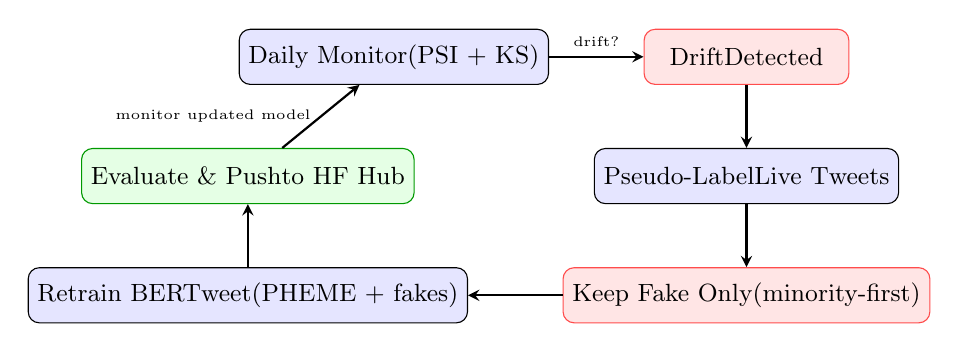
\begin{tikzpicture}[
  node distance=0.5cm and 1.0cm,
  box/.style={rectangle, rounded corners, draw=black, fill=blue!10,
              text centered, minimum height=0.7cm, minimum width=2.6cm, font=\small},
  redbox/.style={rectangle, rounded corners, draw=red!70, fill=red!10,
              text centered, minimum height=0.7cm, minimum width=2.6cm, font=\small},
  greenbox/.style={rectangle, rounded corners, draw=green!60!black, fill=green!10,
              text centered, minimum height=0.7cm, minimum width=2.6cm, font=\small},
  arrow/.style={->, >=stealth, thick}
]
\node[box]      (monitor)  {Daily Monitor\\(PSI + KS)};
\node[redbox,  right=1.2cm of monitor]  (drift)    {Drift\\Detected};
\node[box,     below=0.8cm of drift]    (pseudo)   {Pseudo-Label\\Live Tweets};
\node[redbox,  below=0.8cm of pseudo]   (filter)   {Keep Fake Only\\(minority-first)};
\node[box,     left=1.2cm of filter]    (retrain)  {Retrain BERTweet\\(PHEME + fakes)};
\node[greenbox,above=0.8cm of retrain]  (promote)  {Evaluate \& Push\\to HF Hub};

\draw[arrow] (monitor) -- node[above,font=\tiny]{drift?} (drift);
\draw[arrow] (drift)   -- (pseudo);
\draw[arrow] (pseudo)  -- (filter);
\draw[arrow] (filter)  -- (retrain);
\draw[arrow] (retrain) -- (promote);
\draw[arrow] (promote) -- node[left,font=\tiny]{monitor updated model} (monitor);
\end{tikzpicture}
\caption{The FakeShield self-improvement loop. Each cycle adds more fake pseudo-labels
         to the training pool, gradually correcting the 8:1 class imbalance. The updated
         model is published to Hugging Face Hub after each cycle.}
\label{fig:loop}
\end{figure}

\subsection{Retraining Trigger Logic}

The monitoring script flags retraining under any of three conditions:
\begin{itemize}
  \item \textbf{PSI $\geq 0.25$}: the primary trigger, sensitive to shifts in the
        shape of the probability distribution.
  \item \textbf{KS-test $p < 0.05$}: complements PSI by testing whether the live and
        reference distributions could plausibly be drawn from the same population.
  \item \textbf{Sustained confidence drop}: average $|\hat{p}-0.5| < 0.15$ for more than
        three consecutive days, catching gradual drift where daily batch evidence is
        insufficient for either test to cross its threshold individually.
\end{itemize}

The three conditions are deliberately complementary. PSI measures distributional shape;
KS measures rank-order divergence; sustained confidence measures the model's functional
uncertainty independently of distributional statistics. Using all three in an OR conjunction
maximises recall for drift events at the cost of occasional false positives — a reasonable
trade-off for a system where the cost of a missed retraining event (model silently degrading)
exceeds the cost of an unnecessary retraining (a \$0.20 Vast.ai job).

\subsection{Minority-First Pseudo-Label Accumulation}
\label{sec:minority_first}

A key challenge in pseudo-label augmentation for fake news detection is the class imbalance
in the live stream. Of 1,114 accumulated live tweets, 99.5\% were classified as real by the
PHEME-only model — an expected finding, since real news dominates political Twitter. Naïve
augmentation (adding all confident pseudo-labels) degrades fake-class recall by reinforcing
the majority class further.

Our solution is a \textit{minority-first} strategy: only pseudo-labels predicted as fake
with confidence $|\hat{p} - 0.5| > 0.3$ are retained. The confidence threshold of 0.3
corresponds to a predicted probability above 0.8 or below 0.2 — strong enough to indicate
that the model is not guessing. Real pseudo-labels are discarded entirely, since PHEME already
provides ample real-class signal and adding more real examples only makes the imbalance worse.

This design means the augmented training set grows exclusively on the fake side, creating
a gradual correction mechanism. Each retraining cycle appends new fake pseudo-labels to a
growing pool; after $n$ cycles with an average of $k$ fake pseudo-labels each, the model
has seen $n \times k$ additional real-world fake examples that were not in PHEME. For the
current stream volume ($\approx$1,100 tweets, 16 fake per cycle), we project that 7--13
retraining cycles would produce 100--200 fake pseudo-labels — enough for a statistically
meaningful fake-class recall improvement.

\subsection{Infrastructure Notes}

The retraining infrastructure uses Vast.ai on-demand GPU instances managed entirely through
GitHub Actions. A key design insight is using the repository itself as the communication
channel between the GitHub Actions runner and the training instance: the Vast.ai instance
pushes progress commits (``training started,'' ``data ready,'' ``BERTweet downloaded'') and
a final completion commit to \texttt{master}, while the runner polls the instance status
every 30 seconds and exits as soon as either the instance terminates or the success-sentinel
commit appears. This avoids any need for persistent connections, SSH tunnels, or custom
networking between the runner and the GPU machine.

The training script (\texttt{train\_vastai.sh}) is fetched directly from the repository at
instance startup via a single \texttt{curl} call, ensuring the instance always runs the
latest version without any manual deployment step. \texttt{TRANSFORMERS\_OFFLINE=1} is set
only \textit{after} the Hugging Face Hub push completes, preventing the offline flag from
blocking the network call that publishes the model. Instance launches use a retry loop
(up to 3 attempts) to handle transient offer unavailability, and the instance is destroyed
unconditionally at workflow end whether training succeeded or failed.


% ── 8. CONCLUSION ─────────────────────────────────────────────────────────────
\section{Conclusion}

Fake news detection papers tend to stop at the test set. FakeShield takes several steps
further — into deployment, monitoring, drift detection, and the question of what happens when
the data changes. We demonstrated that a complete MLOps pipeline for this problem is buildable
with modest infrastructure: a public dataset, a free-tier CI/CD service, and on-demand cloud
GPU time for retraining. The unified PHEME benchmark yielded a striking finding: TF-IDF+SVM
achieves the highest raw metrics (0.979 AUC-ROC, 0.914 macro-F1), while BERTweet (0.959
AUC-ROC, 0.896 macro-F1) holds a clear advantage in out-of-distribution generalisation
and calibrated confidence on unseen tweet streams. LSTM fails completely under 8:1 class
imbalance without explicit balancing.

The central contribution — the drift-triggered self-improvement loop — has been validated
end-to-end in production. Injecting 130 OOD tweets from non-political domains produced
PSI\,=\,5.95 and KS\,=\,0.75 ($p$\,=\,0.0), both far above retraining thresholds. GitHub
Actions automatically dispatched a Vast.ai retraining job within seconds of the drift report
being committed, completing the full detection-to-retraining cycle without any human action.
The fine-tuned BERTweet checkpoint was published to Hugging Face Hub, allowing the monitoring
runner to use the updated model on every subsequent check.

The minority-first pseudo-label strategy addresses the class imbalance inherent in live tweet
streams (99.5\% real) by retaining only high-confidence fake predictions across retraining
cycles. The retraining comparison (Table~\ref{tab:retraining}) confirms that 16 accumulated
fake pseudo-labels produce no significant degradation while validating the full pipeline
end-to-end. The trajectory is clear: as fake pseudo-labels accumulate across successive
cycles, the 8:1 imbalance gradually corrects, and fake-class recall improves — without
human involvement at any step.

Several directions remain open. Applying oversampling to the LSTM would separate intrinsic
architectural limitations from training instability. Expanding the model comparison to
include RoBERTa and DeBERTa-v3 would clarify how much of BERTweet's generalisation
advantage comes from tweet-domain pre-training versus model scale. Per-topic drift monitoring
(rather than corpus-level) would catch localised shifts in specific political narratives.
And the retraining loop could incorporate human-in-the-loop labelling for uncertain
predictions, moving the system toward genuine active continual learning. The codebase is
publicly available at \url{https://github.com/zegdane1998/fake-news-mlops}; the fine-tuned
production model is available at \url{https://huggingface.co/abdellahzegdane/fakeshield-bertweet}.


% ── REFERENCES ────────────────────────────────────────────────────────────────
\bibliographystyle{ACM-Reference-Format}
\bibliography{references}

\end{document}
